\documentclass{article}  
\usepackage[utf8]{geometry}
\geometry{a4paper,12pt, scale=0.8}
\renewcommand*\familydefault{\sfdefault}
\usepackage[scaled]{helvet}
\renewcommand\familydefault{\sfdefault} 
\usepackage[T1]{fontenc}
\usepackage{listings}
\usepackage{color}
\usepackage{graphicx}

\definecolor{dkgreen}{rgb}{0,0.6,0}
\definecolor{gray}{rgb}{0.5,0.5,0.5}
\definecolor{mauve}{rgb}{0.58,0,0.82}

\lstset{frame=tb,
  language=C,
  aboveskip=3mm,
  belowskip=3mm,
  showstringspaces=false,
  columns=flexible,
  basicstyle={\small\ttfamily},
  numbers=none,
  numberstyle=\tiny\color{gray},
  keywordstyle=\color{blue},
  commentstyle=\color{dkgreen},
  stringstyle=\color{mauve},
  breaklines=true,
  breakatwhitespace=true,
  tabsize=3
}
\title{CS2002-P4-Report}
\author{170011474}
\date{2019 April}
\begin{document}  
\maketitle

\section{Overview}
This practical exposes system library tools for multi-process, multi-threaded, and elements of concurrent programming. The task 1 requires students to implement 10 chain children and each child will modify the string by swapping indices. Task 2 requires students to draw a diagram to show the relationships between threads with "create" and "join" labelled. 
\section{Task 1: The Telephone Game}
There is only one source file containing all codes for task 1: \texttt{rumours.c}. \texttt{main()} is implemented as the entry point to process input and invoke other functions. \textbf{I added an additional extension to this task apart: rather than randomly swapping two letters, this program will reverse the whole string by swapping two letters for each process.} For example, "abcd" will be reversed as "dcba". I found this small modification is much more interesting than randomly swapping. 
\subsection{Design \& Implementation}
\paragraph{Obtain input string from stdin. }
malloc() and realloc() have been used. In this way, we do not have to assume a length for the input string. Therefore, the waste of space will be avoided and memory space is used efficiently. By iterating over the arguments array, the token of the string will be appended to the current string, with space separated. Eventually, this string can be treated as the input and be passed to other functions.
\paragraph{Recursion to create child processes: getNewChild().}
Since students are supposed to create 10 chain processes, so a threshold for "10" is required for the base case. When the current depth is 0, then the function should terminate immediately. getNewCHild() will be called after a child process fulfils its own tasks, and new child is created. The original child process becomes a parent process with its new function to be performed again.
\begin{lstlisting}
	printf("New process: %i, parent: %i \n", getpid(), getppid());
	printf("pid: %i received string: %s \n", getpid(), buffer);
	getNewChild(file, buffer, depth - 1, len, index + 1);
\end{lstlisting}
The depth indicates the current depth. \textit{Note that it should be subtracted by 1 when a new getNewChild() is called.}
\paragraph{Pipe between parent and child processes.}
Parent processes modify the string by swapping two letters, and then write the new string to the pipe. From the other side, the child processes receive string and prompt proper messages in stdout. Note that pipe() should be called before a child is forked.
\paragraph{Another way to implement: Exit parent process for each time.} Although I used recursion to realise the functionality, I have also written codes without recursion to implement it. The biggest problem is that every time a new iteration begins, the old parent process will disturb the new parent and the new child process more or less. So at the end of the parent block, parent can call exit() to exit itself. I succeeded to run it but I tried to use recursion since my recursive thinking needs to be strengthened. The original codes for this "no recursion" way were lost and there is no time for me to write them again. Otherwise, two different ways can be displayed in this coursework.
\subsection{Testing (basic)}
When the input is "i love fish and chips", we can see this string is reversed as "spihc dna hsif evol i". Also, the process id goes from 13060 to 13070, forming a one-child family tree.
\begin{lstlisting}
	pid: 13060 Swapped indices 0, 20 
	New process: 13061, parent: 13060 
	pid: 13061 received string: s love fish and chipi  
	pid: 13061 Swapped indices 1, 19 
	New process: 13062, parent: 13061 
	pid: 13062 received string: splove fish and chi i  
	pid: 13062 Swapped indices 2, 18 
	New process: 13063, parent: 13062 
	pid: 13063 received string: spiove fish and chl i  
	pid: 13063 Swapped indices 3, 17 
	New process: 13064, parent: 13063 
	pid: 13064 received string: spihve fish and col i  
	pid: 13064 Swapped indices 4, 16 
	New process: 13065, parent: 13064 
	pid: 13065 received string: spihce fish and vol i  
	pid: 13065 Swapped indices 5, 15 
	New process: 13066, parent: 13065 
	pid: 13066 received string: spihc  fish andevol i  
	pid: 13066 Swapped indices 6, 14 
	New process: 13067, parent: 13066 
	pid: 13067 received string: spihc dfish an evol i  
	pid: 13067 Swapped indices 7, 13 
	New process: 13068, parent: 13067 
	pid: 13068 received string: spihc dnish af evol i  
	pid: 13068 Swapped indices 8, 12 
	New process: 13069, parent: 13068 
	pid: 13069 received string: spihc dnash if evol i  
	pid: 13069 Swapped indices 9, 11 
	New process: 13070, parent: 13069 
	pid: 13070 received string: spihc dna hsif evol i 
\end{lstlisting}
\subsection{Testing (extension)}
When we want to reverse "ab", "ba" is returned and there are only 2 processes needed to reverse it.
\begin{lstlisting}
	pid: 14415 Swapped indices 0, 1 
	New process: 14416, parent: 14415 
	pid: 14416 received string: ba 
\end{lstlisting}
As the specification sheet mentioned, \textbf{the changed strings should appear in the reverse order from which they were generated in a file rumours.out}. So the result in the rumours.out shows as below: 
\begin{lstlisting}
	pid: 14452 received string: spihc dna hsif evol i  
	pid: 14451 Swapped indices 9, 11 
	pid: 14451 received string: spihc dnash if evol i  
	pid: 14450 Swapped indices 8, 12 
	pid: 14450 received string: spihc dnish af evol i  
	pid: 14449 Swapped indices 7, 13 
	pid: 14449 received string: spihc dfish an evol i  
	pid: 14448 Swapped indices 6, 14 
	pid: 14448 received string: spihc  fish andevol i  
	pid: 14447 Swapped indices 5, 15 
	pid: 14447 received string: spihce fish and vol i  
	pid: 14446 Swapped indices 4, 16 
	pid: 14446 received string: spihve fish and col i  
	pid: 14445 Swapped indices 3, 17 
	pid: 14445 received string: spiove fish and chl i  
	pid: 14444 Swapped indices 2, 18 
	pid: 14444 received string: splove fish and chi i  
	pid: 14443 Swapped indices 1, 19 
	pid: 14443 received string: s love fish and chipi  
	pid: 14442 Swapped indices 0, 20 
\end{lstlisting}
As we can see, changed strings show in the reverse order. So the top string is the reversed string, and the bottom string is the original string from stdin. My personal extension can show this feature in a more straightforward way. 



\section{Task 2: Thread-join Diagram}
In this task, students need to draw a thread-join diagram given the code. The marker can find these codes in "thread1.c" under the same directory. "make" and then "./test" can run this program. \\
\begin{center}
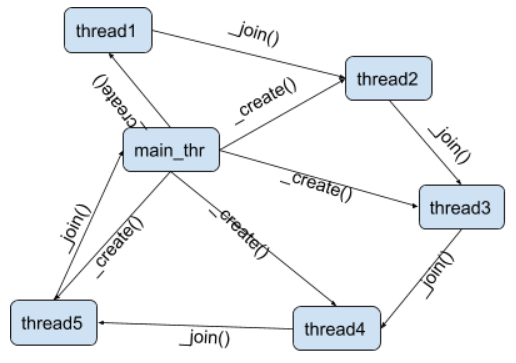
\includegraphics[scale=0.5]{diagram.png}
\end{center}
\paragraph{Explanation.}
main() creates 5 threads in total, storing them in the \texttt{pthread\_t thread}. When the \texttt{pthread\_create()} is called, the current thread id will overwrite the \texttt{thread}, with the thread value treated as an argument passed by the function \texttt{worker()}. 
\paragraph{\_create()}
As all 5 threads are created by the for loop, and the for loop locates in the main() which indicates the \texttt{main\_thread} (main\_thr in the diagram) has created them all. That is why all \texttt{\_created()} point to the threads from the \texttt{main\_thr}.
\paragraph{\_join()}
The most important part is the \_join() part. The diagram shows that the "elder" thread (i.e. thread 1) is joined by the more recent thread (i.e. thread 5). And the most recent thread which is thread 5 is joined by the \texttt{main\_thr}.

\subsection{Justification}
I have added another line of code to print out the current index and the current thread id as below: 
\begin{lstlisting}
	for(int i = 0; i < 5; i++){
        // print out the current index and the current thread
        printf("the %i iteration %u thread\n", i, thread);
        pthread_create(&thread, NULL, worker, (void *)thread);
    }
\end{lstlisting}
And the result shows below:
\begin{lstlisting}
	the main thread 1804773184 
	the 0 iteration 0 thread
	the 1 iteration 1804769024 thread
	the 2 iteration 1796376320 thread
	the 3 iteration 1787983616 thread
	the 4 iteration 1779590912 thread
	the 5 iteration 1771198208 thread
\end{lstlisting}
\emph{Note that the 0 iteration 0 thread is because the \texttt{thread} was initialised as "NULL" at the time, which will be displayed as "0".}
\paragraph{From here we can see thread ids from the oldest thread (thread 1) to the newest thread (thread 5).} Print out the current thread ids and the joined thread ids as below:
\begin{lstlisting}
	if(data){
        printf("current: %u, joins: %u \n", pthread_self(), (pthread_t)data);
        pthread_join((pthread_t)data, NULL);
    }
\end{lstlisting}
\begin{lstlisting}
	current: 1796376320, joins: 1804769024 
	current: 1787983616, joins: 1796376320 
	current: 1779590912, joins: 1787983616 
	current: 1771198208, joins: 1779590912 
	current: 1804773184, joins: 1771198208
\end{lstlisting}
According to the thread ids, it is:  
\begin{lstlisting}
	current: thread2, joins: thread1 
	current: thread3, joins: thread2 
	current: thread4, joins: thread3 
	current: thread5, joins: thread4
	current: main_thread, joins: thread5
\end{lstlisting}
So here we can know the diagram displays the relationships correctly.

\section{Task 3 (Extension): A real "Shadow Breaker"}
For this task, students are expected to recover the password given a hash and a prefix of the password. 
\subsection{Design & Implementation}
\paragraph{Use a struct type "Info" to contain necessary arguments, passed to functions.} The \texttt{thread\_start\_routine()} only accepts one \texttt{void *} argument, while there are many arguments needed, so a struct can be the media to send those information as an entire instance. \texttt{Info} contains \texttt{username, pw\_hash, pw\_prefix, thread\_count, id, success}. What has to be mentioned is that the success is a flag to represent the state: whether there is a thread that succeed to recover the original password. If not, success as a Integer will remain "0". When a thread succeeds, it will change the success from 0 to 1. Each threads will check the state of success before each iteration. This implementation can save a lot of time and space, to return the genuine password quickly.

\paragraph{How to encrypt the hash? }
The fundamental implementation is that:
\begin{enumerate}
	\item  For each thread, set up the subrange firstly, and then get \texttt{start\_password0} based on the \texttt{start\_index} provided by \texttt{getSubrange()}. For example, the first thread for "abcdef.." has the start\_password "abcdefaa".
	\item Hash the current \texttt{start\_password}, and then compare the temporary hash with the given hash. If they are the same as each other, then the current start\_password is the genuine password.
	\item If they do not match with each other, then use \texttt{incrementString()} to make a new trial. For example, if "abcdefaa" fails, then increments it and "abcdedab" is our new \texttt{start\_password}. We only need to increment the current string based on our \texttt{start\_password}. 
	\item Do step 2, 3, 4 until we get the same hash. Then we return the current \texttt{start\_password} and set up the global \texttt{password} variable. Change the success state so other threads will terminate.
\end{enumerate} 
Here is the basic for loop for step 2, 3, 4.
\begin{lstlisting}
	for (int i = 0; i < count; i++)
  	{
    	if (user->success == 1)
      		break;
    	struct crypt_data temp_data;
    	temp_data.initialized = 0;
    	const char *hashed_temp = crypt_r(start_password, salt_str, &temp_data);
    	hash_count++; // the current iterations we have done

    	if (strcmp(pw_hash, hashed_temp) == 0)
    	{ // if the trial password matches
      		setPassword(strlen(start_password), start_password); // to return it later
      		result_for_print = 0; // for print_thread_parr_result()
      		user->success = 1; // update the flag to let other threads know
      		break;
    	}		
    	incrementString(start_password); // if not match, increment it for a new trial
  	}
\end{lstlisting}

\paragraph{How can you get start\_password?}
To obtain a \texttt{start\_password}, we need a \texttt{start\_index}, a \texttt{const char *prefix}, a \texttt{unknown\_count}(number of unknown letters). Since the prefix is \texttt{const char}, which can not be modified for security, a new string is needed. So I used \texttt{malloc()} to allocate memory space for the \texttt{start\_password} with the same length of the prefix. Then the known prefix will be put into it. A new string for the rest of unknown letters is created, which is initialised by "a" for each element. The \texttt{setStringPosition()} will be only applied on the array of unknown letters and then the array of unknown letters will be concatenated to the prefix. The reason I did not directly use setStringPosition() for the prefix is that \texttt{start\_index} might change the original prefix if it is a wrong index. 

\paragraph{Difficulty: How to print summary correctly after all threads return?}
The problem I found is that when one thread finds the password and lets other threads know, the main thread probably prints out the summary before other threads terminate. I chose to use \texttt{sleep()} before the summary method, while the sleeping seconds matters particularly in different running environments. This is not stable or safe enough. So I used a for loop to join all threads right after the for loop to create these threads. In this way, the main thread will wait until all threads are joined, and then the summary method can perform its function in the correct routine.


\subsection{Testing}
\subsubsection{Testing 1 (2 threads)}
The running result for password "cdmziclt", with given prefix "cdmzi".
\begin{lstlisting}
	Start u000000
	Thread 4156401408: Start u000000 at 0 (cdmziaaa)
	Thread 4156401408: Stop after 1658 iterations (found)
	Thread 4148008704: Start u000000 at 8788 (cdmzinaa)
	Thread 4148008704: Stop after 0 iterations (cancelled)
	Password for u000000 is cdmziclt (1658 hashes in 2.00 seconds)
	Total CPU time: 0.01 seconds.
	CPU usage: 0.01x
\end{lstlisting}
We can see from the above results, each thread starts from their correct start\_index and has equal part of tasks to finish. Also, if one thread succeeds, then other threads will print either "end" or "cancelled". Requirements are satisfied. 
\subsubsection{Testing 2 (4 threads)}
4 threads.
\begin{lstlisting}
	@pc2-013-l:~/CS2002/Practicals/Practical4/shadowbreaker $ ./shadow_breaker 4 < pwd_hashes.txt

	Start u000000
	Thread 362592000: Start u000000 at 0 (cdmziaaa)
	Thread 362592000: Stop after 1658 iterations (found)
	Thread 354199296: Start u000000 at 4394 (cdmzigna)
	Thread 354199296: Stop after 0 iterations (cancelled)
	Thread 345806592: Start u000000 at 8788 (cdmzinaa)
	Thread 345806592: Stop after 0 iterations (cancelled)
	Thread 268433152: Start u000000 at 13182 (cdmzitna)
	Thread 268433152: Stop after 0 iterations (cancelled)
	Password for u000000 is cdmziclt (1658 hashes in 4.00 seconds)
	Total CPU time: 0.01 seconds.
	CPU usage: 0.00x
\end{lstlisting}

\subsubsection{Testing 3 (invalid input)}

When a user is trying to have more than 13 threads, then a proper warning will prompt out: 
\begin{lstlisting}
	@pc2-013-l:~/CS2002/Practicals/Practical4/shadowbreaker $ ./shadow_breaker 15 < pwd_hashes.txt
	The thread_count should be less than 14 
\end{lstlisting}

When the input username has more than 8 letters (username is u0000000000): 
\begin{lstlisting}
	@pc2-013-l:~/CS2002/Practicals/Practical4/shadowbreaker $ ./shadow_breaker 1 < pwd_hashes.txt
	the length of username should be between 1 and 8 
\end{lstlisting}
When the length of the hash is not 13:
\begin{lstlisting}
	@pc2-013-l:~/CS2002/Practicals/Practical4/shadowbreaker $ ./shadow_breaker 1 < pwd_hashes.txt
	the length of hash should be 13 
\end{lstlisting}
When the length of the prefix is not 8:
\begin{lstlisting}
	@pc2-013-l:~/CS2002/Practicals/Practical4/shadowbreaker $ ./shadow_breaker 1 < pwd_hashes.txt
	the length of prefix should be 8
\end{lstlisting}
\section{Evaluation \& Conclusion}
During this practical, I gained deeper insights in the process-processing and thread-processing. 
\begin{itemize}
	\item Codes are clear and simple to follow, with sufficient comments and explanation.
	\item Requirements are satisfied.
	\item Tests have been written to guarantee the functionality.
	\item Justification is provided.
\end{itemize}

\end{document}